\documentclass[12pt]{book}
\let\cleardoublepage\clearpage
\usepackage[utf8]{inputenc}
\usepackage{lmodern}
\usepackage[spanish,es-tabla]{babel}
\usepackage{amsmath}
\usepackage{amsfonts}
\usepackage{amssymb}
\usepackage{color}
\usepackage{textcomp}
\usepackage[T1]{fontenc}
\usepackage{graphicx}
\usepackage{makeidx}
\makeindex
\usepackage{anysize}
\usepackage{anyfontsize}
\usepackage{pdfpages}
\usepackage[x11names,table]{xcolor}
\usepackage{tikz}
\usepackage{tcolorbox}
\usepackage[hidelinks]{hyperref}
\usepackage{caption}
\usepackage{listings}
\usepackage[left=2cm,top=2cm,right=2cm,bottom=2cm]{geometry}
\setlength{\parindent}{0cm}
\tcbset{colback=green!5!white, colframe=gray!10!black, coltitle=green!20!black, 
fonttitle=\bfseries, colbacktitle=white, coltext=gray!30!black}
\usepackage{epigraph}
\usepackage[printwatermark]{xwatermark}
\usepackage{xcolor}
\newwatermark[allpages,color=gray!10,angle=45,scale=3,xpos=0,ypos=0]{Borrador}

% Colores
\definecolor{verdep}{rgb}{0.5,0.5,0.9}
\definecolor{ccap}{rgb}{0.2,0.2,0.2}
\definecolor{csec}{rgb}{0.4,0.4,0.4}
\definecolor{csubsec}{rgb}{0.6,0.6,0.6}
\definecolor{cenun}{rgb}{0.2,0.2,0.3}
\definecolor{csol}{rgb}{0.2,0.8,0.1}
\definecolor{backcode}{rgb}{0.95,0.95,0.99}
\definecolor{dkgreen}{rgb}{0,0.6,0}
\definecolor{gray}{rgb}{0.5,0.5,0.5}
\definecolor{mauve}{rgb}{0.58,0,0.82}

% Nuevos comandos

\usepackage{titlesec}%--
\newcommand{\hsp}{\hspace{5pt}}
\titleformat{\chapter}[hang]{\huge\bfseries\color{ccap}}
{\hsp{\fontsize{35}{5}\selectfont\thechapter .}\hsp%
\hsp{\fontsize{35}{5}\selectfont}}{5pt}{\huge\bfseries}

\titleformat{\section}[hang]{\normalfont\color{csec}}%
{\filright\large\enspace\thesection\enspace}%
{8pt}{\large\bfseries\filright}%

\titleformat{\subsection}[hang]{\normalfont\color{csec}}%
{\filright\large\enspace\thesubsection\enspace}%
{8pt}{\large\bfseries\filright}%

\newcommand{\enunciado}[1]{{\it \textcolor{cenun}{#1}}\vspace{10pt}}
\newcommand{\sol}{{\textcolor{csol}{Solución.}}\vspace{10pt}}

% Code

\lstnewenvironment{matlab}{\lstset{frame=none,
  backgroundcolor=\color{backcode},
  language=Matlab,
  aboveskip=3mm,
  belowskip=3mm,
  showstringspaces=false,
  columns=flexible,
  basicstyle={\small\ttfamily},
  numbers=none,
  numberstyle=\tiny\color{gray},
  keywordstyle=\color{blue},
  commentstyle=\color{dkgreen},
  stringstyle=\color{mauve},
  breaklines=true,
  breakatwhitespace=true,
  tabsize=3,
  extendedchars=true,
  inputencoding=utf8,
  literate=%
  {°}{{\,\,$^\circ$\,\,}}1
  {á}{{\'a}}1
  {é}{{\'e}}1
  {í}{{\'i}}1
  {ó}{{\'o}}1
  {ú}{{\'u}}1
  {Á}{{\'A}}1
  {É}{{\'E}}1
  {Í}{{\'I}}1
  {Ó}{{\'O}}1
  {Ú}{{\'U}}1
}}{}

\author{Pedro Jorge De Los Santos}
\title{Ejercicios resueltos de programación en MATLAB}

\begin{document}
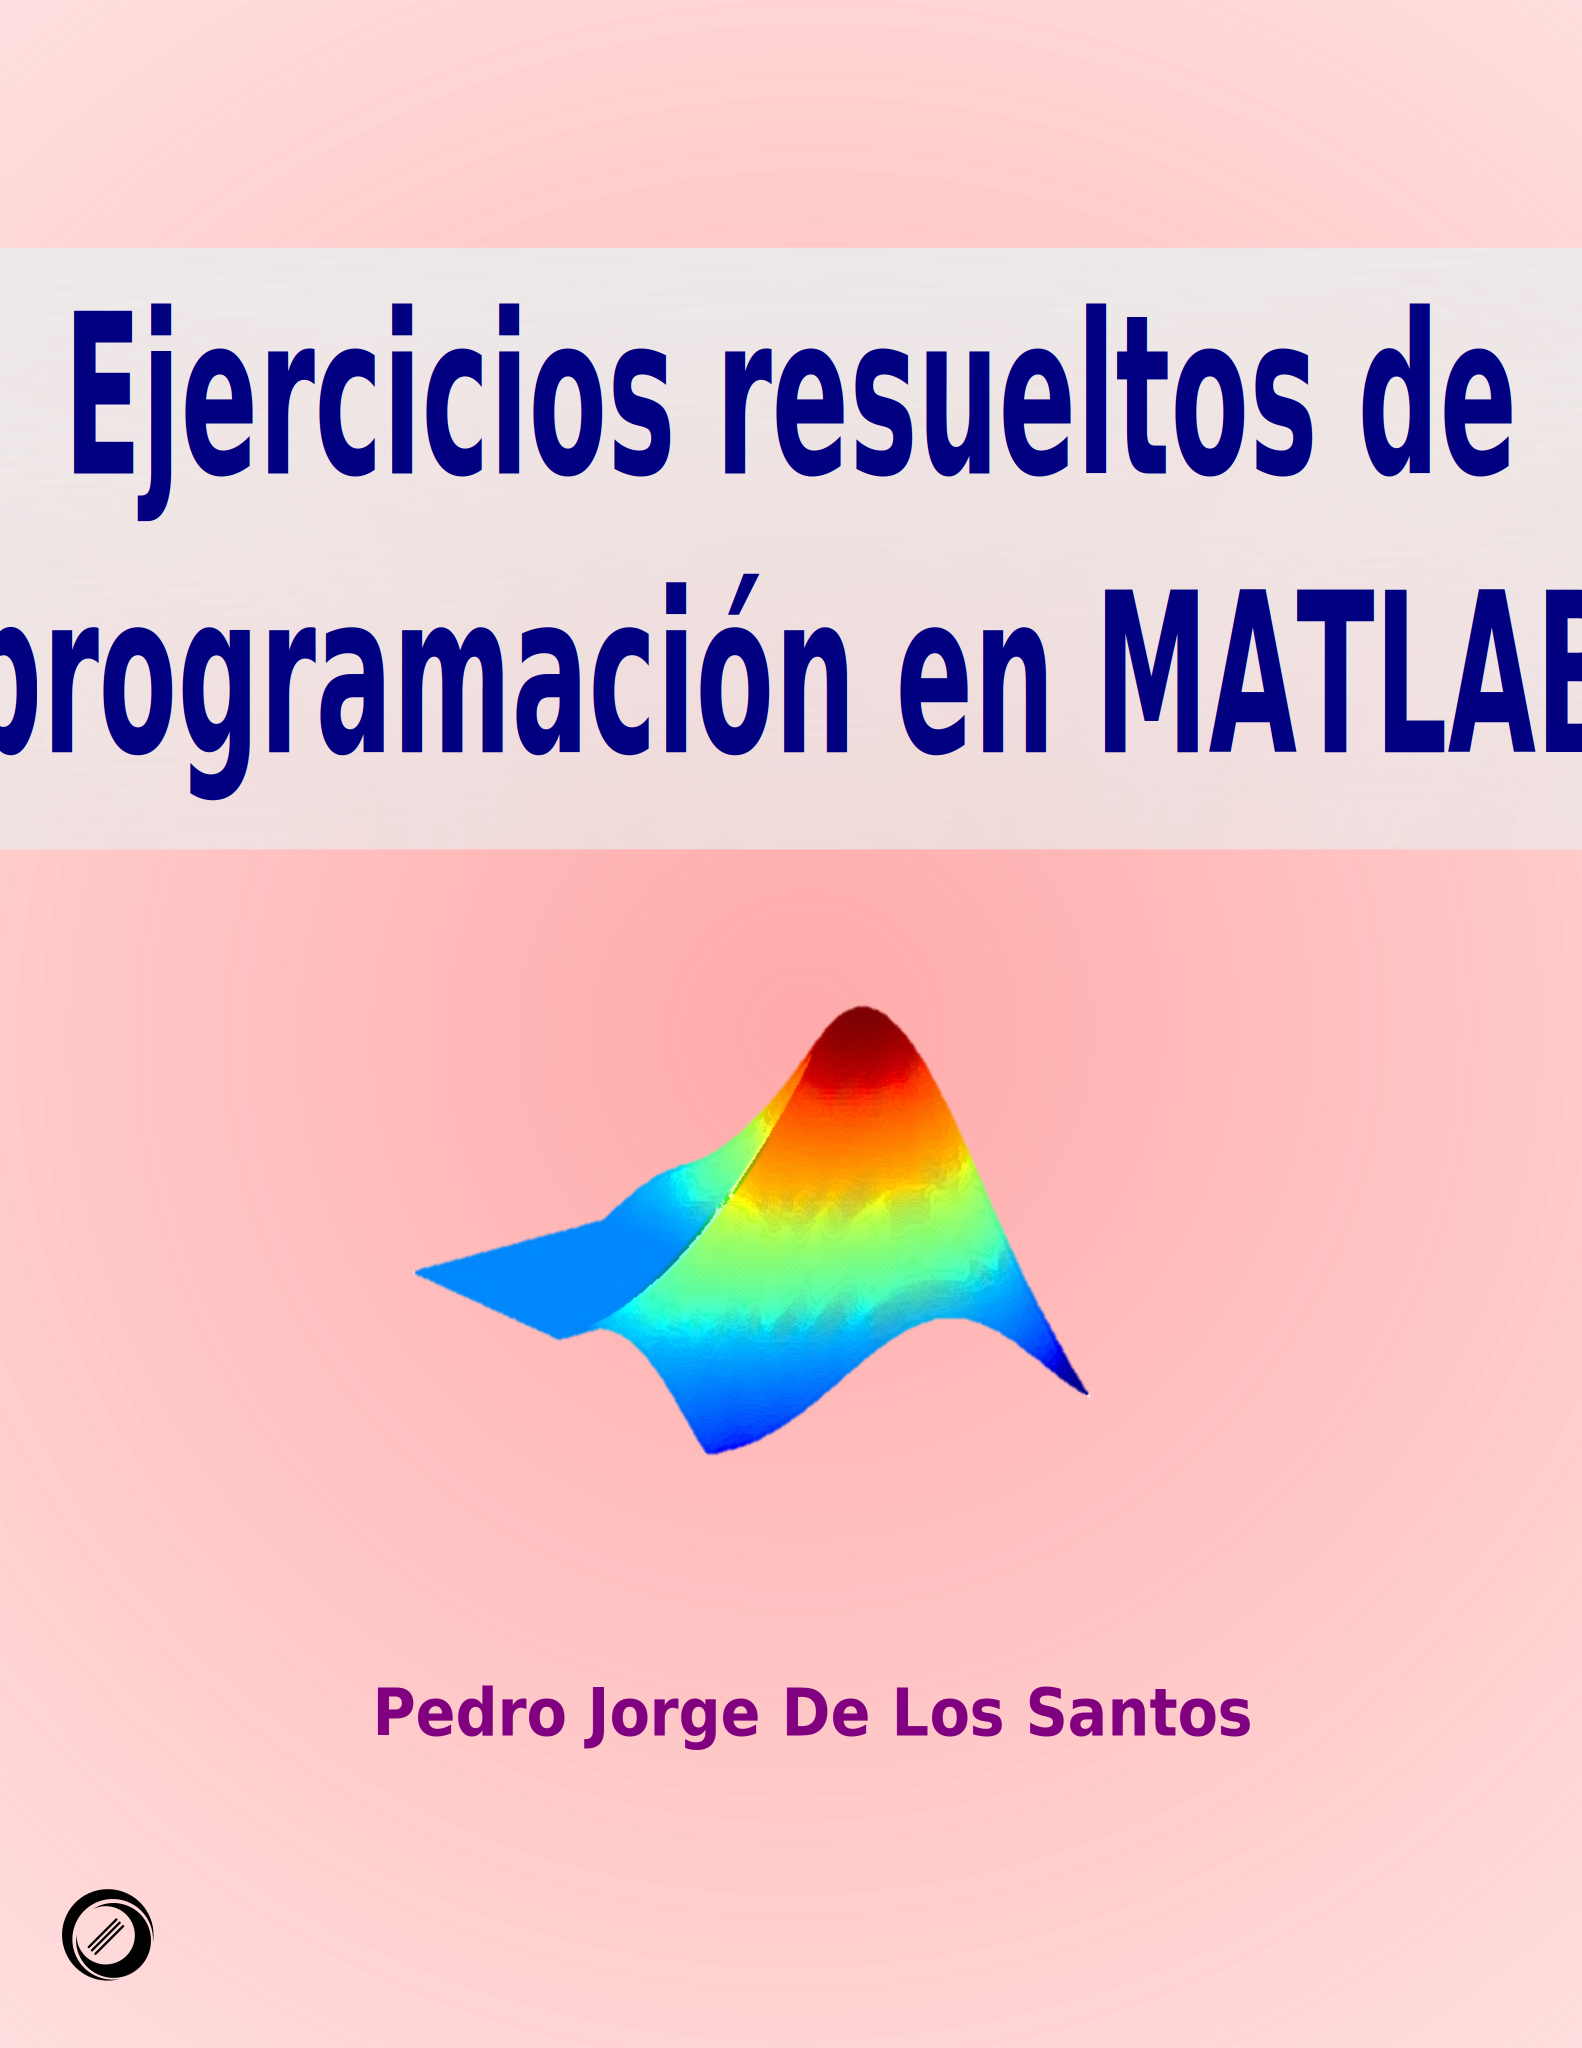
\includepdf{src/portada}
\maketitle
\tableofcontents

% Contenido

% Programación básica
% Matrices y vectores
% Cadenas de caracteres
% Gráficas
% Matemáticas
% GUIs
% POO

\chapter*{Acerca de...}

Este pequeño \textit{libro} se ha escrito con la finalidad de aportar una herramienta auxiliar a la comunidad 
hispanohablante de MATLAB. Orientado, sobre todo, a quienes dan los primeros pasos en la programación 
con este entorno de desarrollo.\\

Los problemas se han clasificado en diversas temáticas, para facilitar el estudio de los mismos. 
Todos los códigos de este libro están disponibles en el siguiente repositorio de GitHub: 
\href{https://github.com/JorgeDeLosSantos}{\bfseries\color{mauve} ERPM}.\\

El autor agradece cualquier tipo de comentario, observación u opinión, y puede remitirla 
a la dirección de correo electrónico que se adjunta posteriormente, o bien, contactándonos 
a través de las diversas plataformas cuyos enlaces se incluyen en la parte inferior.\\ \\

\texttt{Pedro Jorge De Los Santos}\\
\texttt{delossantosmfq@gmail.com}\\

\href{https://labdls.blogspot.mx}{\includegraphics[scale=0.1]{src/blogger_logo.png}}
\href{https://www.youtube.com/user/lab2dls}{\includegraphics[scale=0.1]{src/youtube_logo.png}}
\href{https://github.com/JorgeDeLosSantos}{\includegraphics[scale=0.08]{src/github_logo.png}}
\href{https://www.linkedin.com/in/pjdlsl}{\includegraphics[scale=0.1]{src/linkedin_logo.png}}
\href{https://plus.google.com/u/0/+pjdelossantos}{\includegraphics[scale=0.1]{src/google_logo.png}}
\input{src/parte1.tex}
\input{src/parte2.tex}
\input{src/parte3.tex}
\input{src/parte4.tex}
\input{src/parte5.tex}
\input{src/parte6.tex}
\input{src/parte7.tex}

%\printindex

\end{document}
